\chapter{Proposal For Solution}
\label{proposedSolution}
\begin{enumerate}
    \item 64 i2c nodes housing a ATTINY1617 using its analog comarators to decode RFID signals, each with their own coil and resonance circuit.
    \item Here the i2c bus should not have more than 400pF capasitance in the circuit to be stable and readable. I think there are tools for this in Altium.
    \item 1 ATmega4809 controlling the 64 nodes. This will do all the major computing.
    \item RGB leds in every square controlled by a ATmega328, this will light up differently according to the cirumstances.
\end{enumerate}

\begin{figure}[]
    \centering
    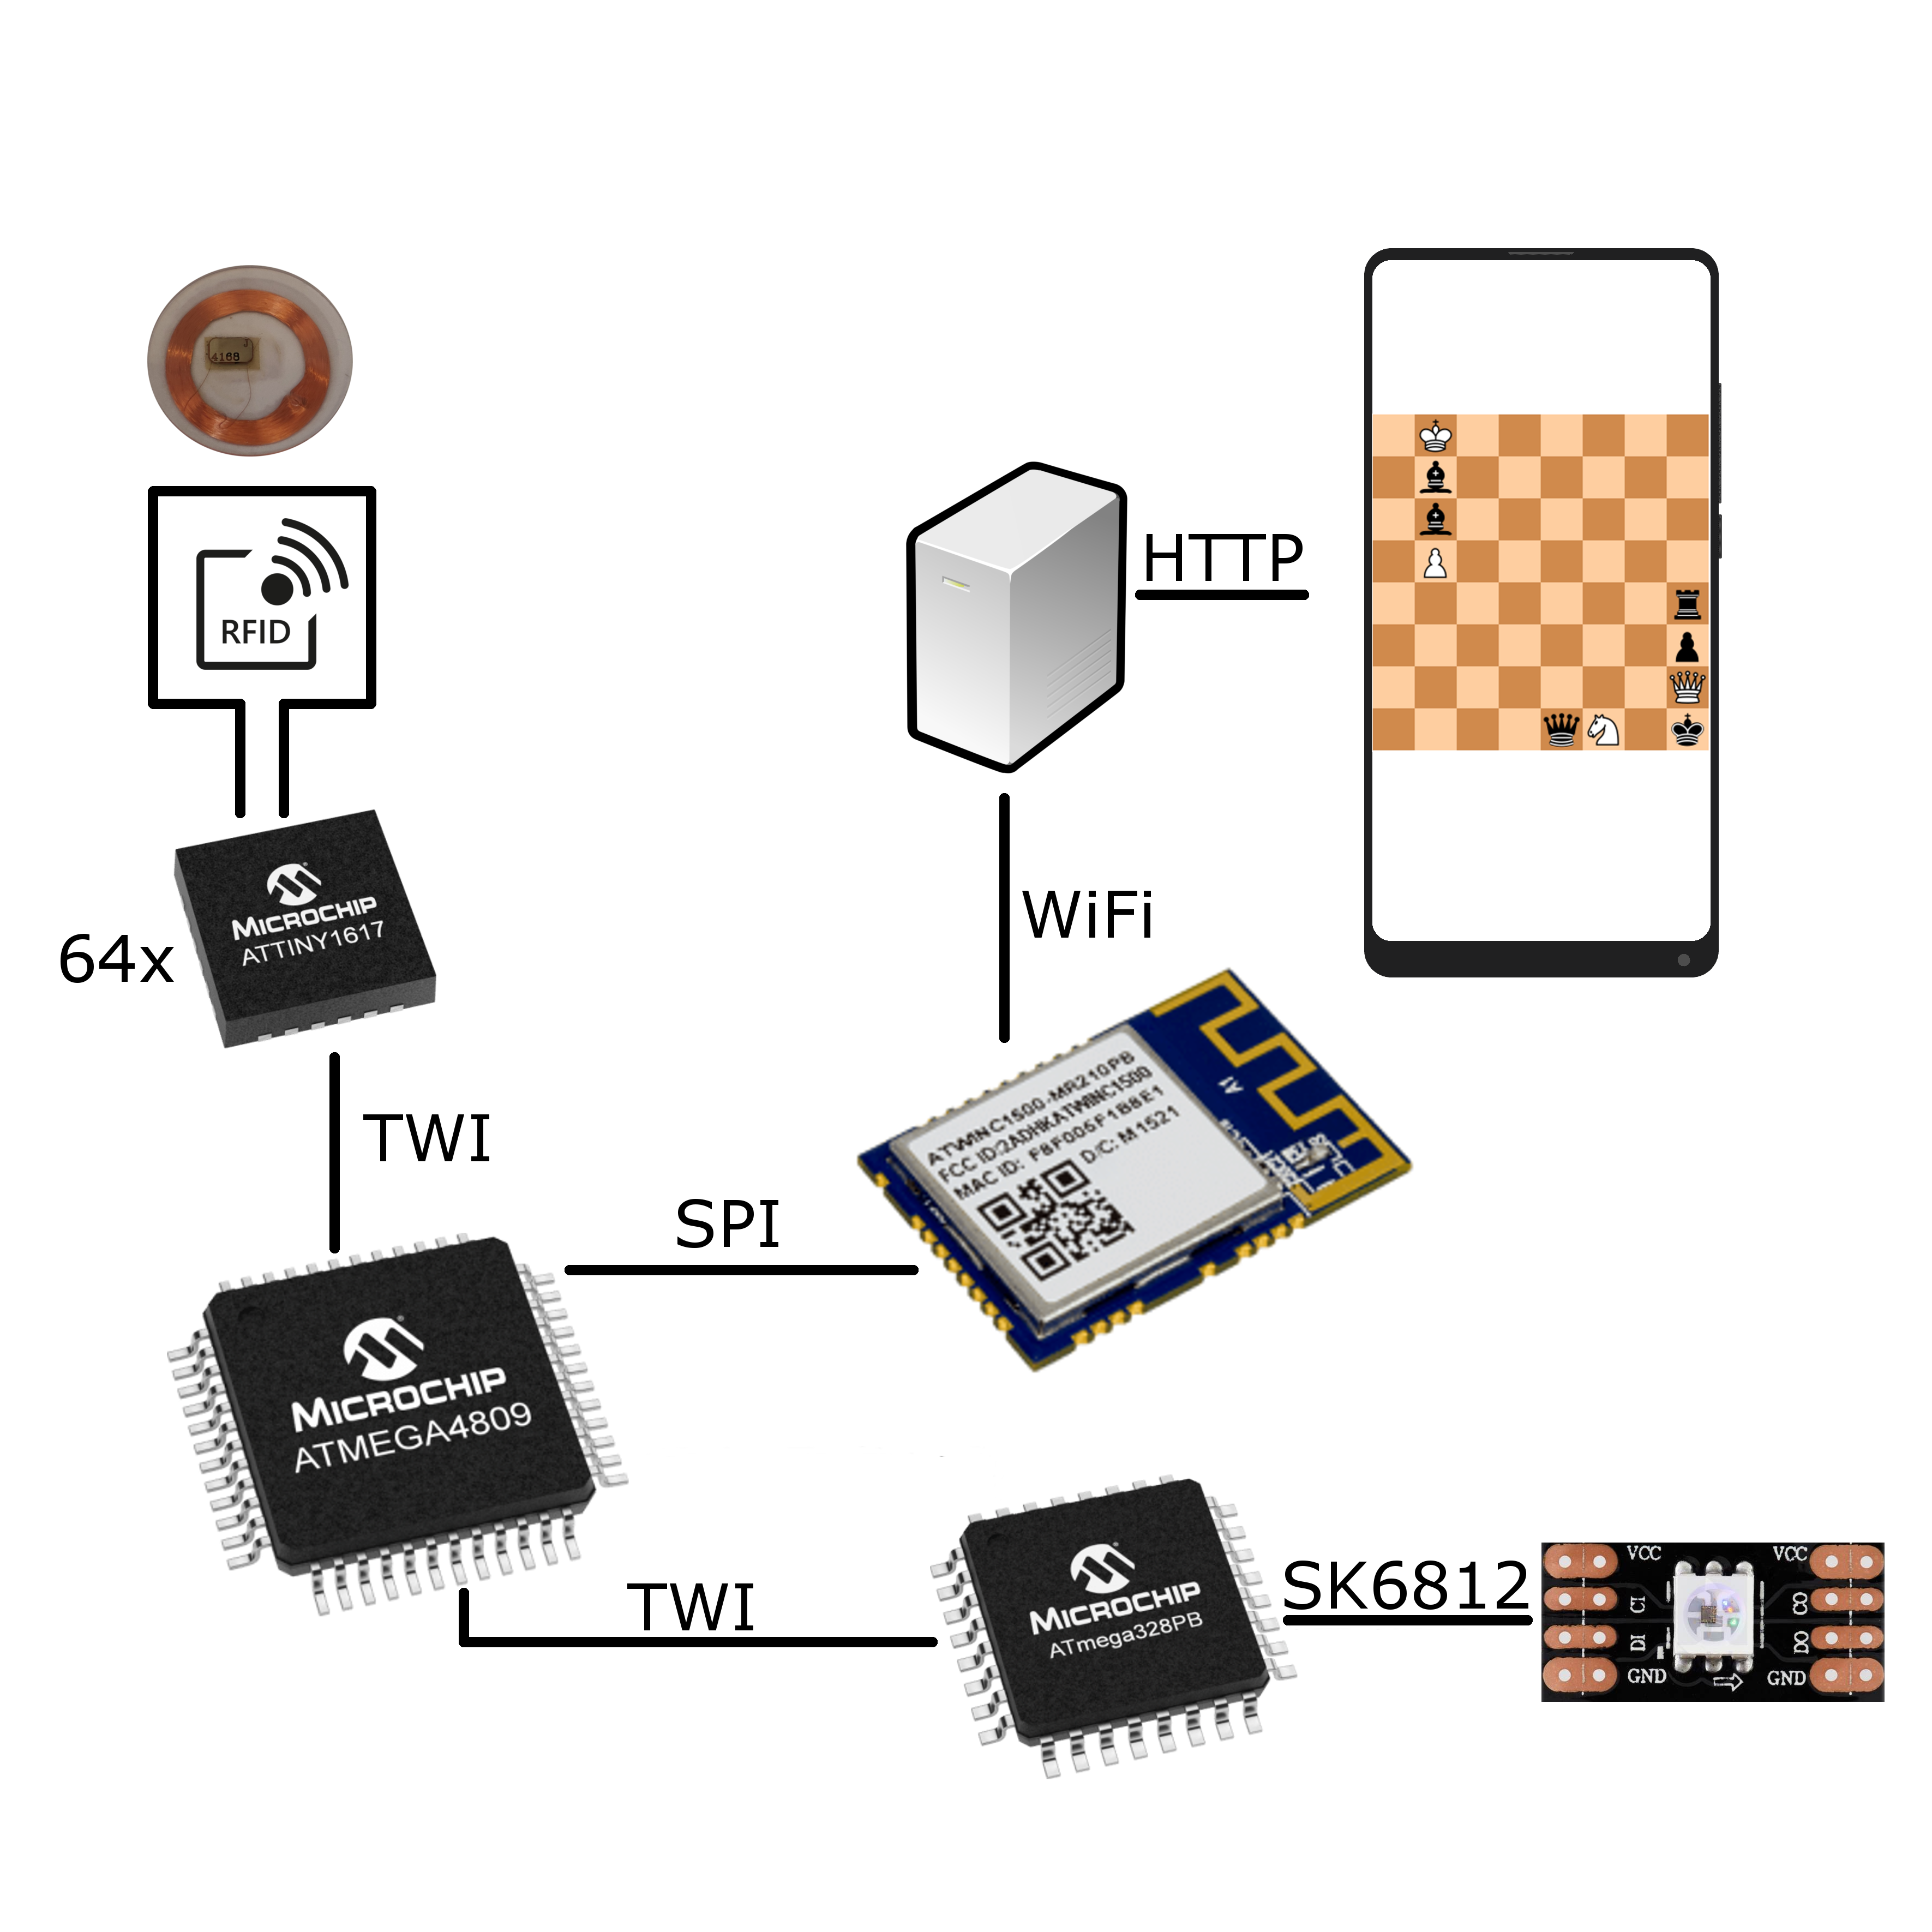
\includegraphics[width=\textwidth]{04_My_Proposal_For_Solution/figures/system_overview.png}
    \caption{Porposed system dataflow}
    \label{fig:04:Dataflow}
\end{figure}
